%**************************************************************************
%* SpringSim 2020 Author Kit
%*
%* Word Processing System: TeXnicCenter and MiKTeX
%*
%**************************************************************************

\documentclass{scspaperproc}

\usepackage{latexsym}
\usepackage{graphicx}
\usepackage{mathptmx}

%
%****************************************************************************
% AUTHOR: You may want to use some of these packages. (Optional)
\usepackage{amsmath}
\usepackage{amsfonts}
\usepackage{amssymb}
\usepackage{amsbsy}
\usepackage{amsthm}
%****************************************************************************


%
%****************************************************************************
% AUTHOR: If you do not wish to use hyperlinks, then just comment
% out the hyperref usepackage commands below.

%% This version of the command is used if you use pdflatex. In this case you
%% cannot use ps or eps files for graphics, but pdf, jpeg, png etc are fine.

\usepackage[pdftex,colorlinks=true,urlcolor=blue,citecolor=black,anchorcolor=black,linkcolor=black,bookmarks=false]{hyperref}

%% The next versions of the hyperref command are used if you adopt the
%% outdated latex-dvips-ps2pdf route in generating your pdf file. In
%% this case you can use ps or eps files for graphics, but not pdf, jpeg, png etc.
%% However, the final pdf file should embed all fonts required which means that you have to use file
%% formats which can embed fonts. Please note that the final PDF file will not be generated on your computer!
%% If you are using WinEdt or PCTeX, then use the following. If you are using
%% Y&Y TeX then replace "dvips" with "dvipsone"

%% \usepackage[dvips,colorlinks=true,urlcolor=blue,citecolor=black,%
%% anchorcolor=black,linkcolor=black]{hyperref}

%% The use of the long citation format (e.g. "Brown and Edwards (1993)" rather than "[5]") and at the same
%% time using the hyperref package can lead to hard to trace bugs in case the citation is broken accross the
%% line (usually this will mark the entire paragraph as a hyperlink (clickable) which is easily noticeable and fixed
%% if using colorlinks, but not if the color is black -- as it is now). Worse yet, if a citation spans page boundary,
%% LaTeX compilation can fail, with an obscure error message. Since this depends a lot on the flow of the text
%% and wording, these bugs come and go and can be extremely hard for a beginner to trace. The error
%% message can look like this:
%%
%%    ! pdfTeX error (ext4): \pdfendlink ended up in different nesting level than \pdfstartlink.
%%    \AtBegShi@Output ...ipout \box \AtBeginShipoutBox 
%%    \fi \fi 
%%    l.174 
%%    ! ==> Fatal error occurred, no output PDF file produced!
%%
%% and can be universally fixed by putting an \mbox{} around the citation in question (in this case, at line 174)
%% and maybe adapting the wording a little bit to improve the paragraph typesetting, which is perhaps not
%% immediately obvious.
%****************************************************************************

%****************************************************************************
%*
%* AUTHOR: YOUR CALL!  Document-specific macros can come here.
%*
%****************************************************************************

% add custom hyphenation rules here
\usepackage{hyphenat}
\hyphenation{op-tical net-works semi-conduc-tor}

% If you use theorems
\newtheoremstyle{scsthe}% hnamei
{8pt}% hSpace abovei
{8pt}% hSpace belowi
{\it}% hBody fonti
{}% hIndent amounti1
{\bf}% hTheorem head fontbf
{.}% hPunctuation after theorem headi
{.5em}% hSpace after theorem headi2
{}% hTheorem head spec (can be left empty, meaning `normal')i

\theoremstyle{scsthe}
\newtheorem{theorem}{Theorem}
\renewcommand{\thetheorem}{\arabic{theorem}}
\newtheorem{corollary}[theorem]{Corollary}
\renewcommand{\thecorollary}{\arabic{corollary}}
\newtheorem{definition}{Definition}
\renewcommand{\thedefinition}{\arabic{definition}}

% avoid overrunning the right margin; you are welcome to remove this, provided that you take care not to overrun the right margin anywhere in your paper
\sloppy

%#########################################################
%*
%*  The Document.
%*
\begin{document}

%***************************************************************************
% AUTHOR: AUTHOR NAMES GO HERE
% FORMAT AUTHORS NAMES Like: Author1, Author2 and Author3 (last names)
%
%		You need to change the author listing below!
%               Please list ALL authors using last name only, separate by a comma except
%               for the last author, separate with "and"


\SCSpagesetup{Lux, Watson, Chang, Xu, Wang, and Hong}

% AUTHOR: Uncomment ONE of these correct conference names.
\def\SCSconferenceacro{SpringSim'20}
%\def\SCSconferenceacro{SummerSim}
%\def\SCSconferenceacro{AutumnSim}
%\def\SCSconferenceacro{PowerPlantSim}

% AUTHOR: Set the correct year of the conference.
\def\SCSpublicationyear{2020}

% AUTHOR: Set the correct month and dates; the dates are separated by a single minus sign
% with no spaces and no leading zeros, the month is a full name (e.g. April) with the first letter
% capitalized. For example, "April 8-13".
\def\SCSconferencedates{May 19-May 21}

% AUTHOR: Set the correct venue in the form "City, State, Country", for example "Los Angeles, CA, USA".
\def\SCSconferencevenue{Fairfax, VA, USA}

% AUTHOR: Enter the title, all letters in upper case
\title{An Algorithm for Constructing Monotone Piecewise \\ Quintic Hermite Interpolating Polynomials}

% AUTHOR: Enter the authors of the article, see end of the example document for further examples
\author{
Thomas C. H. Lux\\
Layne T. Watson\\
Tyler H. Chang\\ [12pt]
Department of Computer Science\\
Virginia Polytechnic Institute and State University $\,$\\
2000 Torgersen Hall, Blacksburg, VA, USA\\
\{tchlux,ltwatson,thchang\}@vt.edu\\
\and
Li Xu\\%
Yueyao Wang\\%
Yili Hong\\ [12pt]
Department of Statistics\\
$\,$ Virginia Polytechnic Institute and State University\\
213 Hutcheson Hall, Blacksburg, VA, USA\\
yilihong@vt.edu\\
}


\maketitle

%% Examples and notes.
%% 
%% \begin{table}[htb]
%%   \centering
%%   \caption{Caption above the table!}\label{tab:example}
%%   \begin{tabular}{r|l}
%%     First & row \\ \hline
%%     second & row \\
%%     third & row \\
%%   \end{tabular}
%% \end{table}
%% 
%% \begin{figure}[htb]
%%   \centering
%%   \includegraphics[width=0.50\textwidth]{path_without_extension}
%%   \caption{Caption below the figure!}\label{fig:example}
%% \end{figure}
%% 
%% \cite{ref}  - Make a citation that is in parenthesis
%% \citeN{ref} - Make a citation out of parenthesis (for noun usage)
%% \shortcite{ref}  - Make a citation for references with >3 authors.
%% \shortciteN{ref} - Make a noun-form citation for references with >3 authors.
%% 
%% 
%% 5 - 12 page paper mandated
%% 150 word abstract
%% 5 keywords maximum


\section*{Abstract}

An algorithm for computing monotone piecewise quintic interpolating
polynomials is proposed. Algebraic constraints for enforcing
monotonicity are provided that align with quintic monotonicity
theory. The algorithm is implemented, tested, and applied to several
sample problems to demonstrate the improved accuracy of piecewise
quintic monotone interpolation compared to the existing piecewise
cubic solution.

\textbf{Keywords:} monotone, spline, Hermite interpolation, quintic polynomial.


\section{Introduction and Motivation}
\label{sec:introduction}


%% \begin{figure}[htb]
%%   \centering
%%   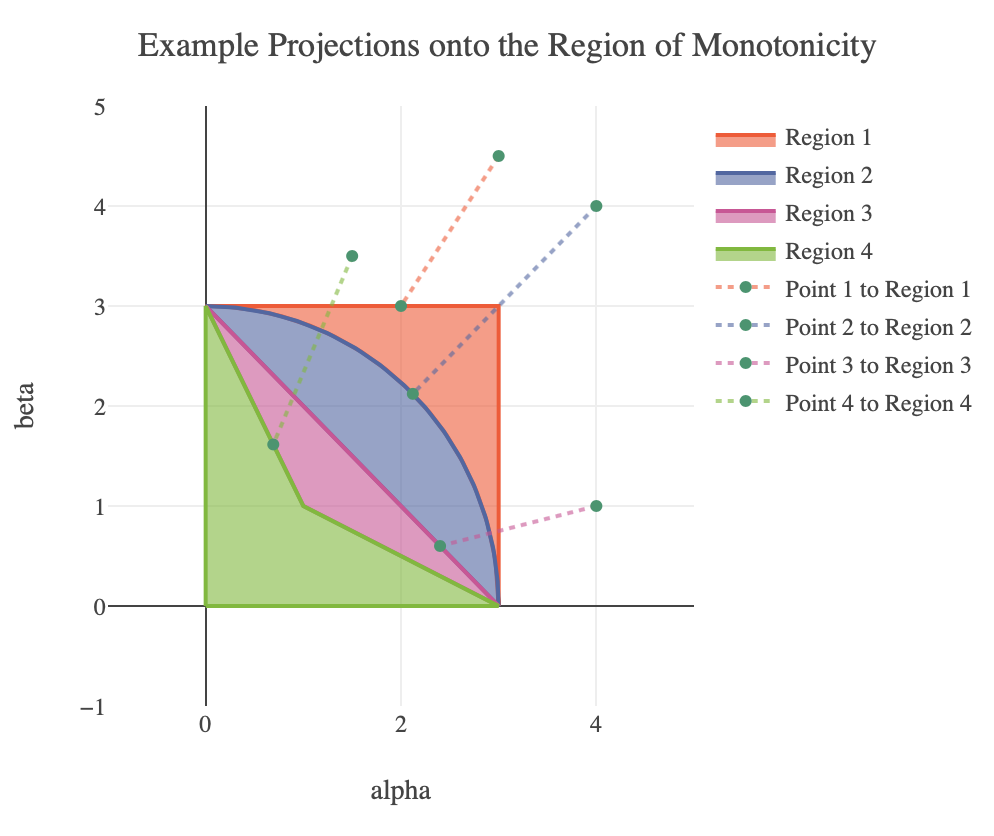
\includegraphics[width=0.50\textwidth]{demo_projection}
%%   \caption{These are the projection mechanisms that make a cubic polynomial piece monotone.}\label{fig:projection}
%% \end{figure}

%% The ability to interpolate or regress a function with continuous value and derivatives has proven fundamentally useful. In many applications, there are known shapes or characteristics that are expected of approximations. For example, a cumulative distribution function in statistics cannot decrease, the entropy of a closed thermodynamic system can never increase, an electric motor should not suddenly change direction when slowing down or speeding up. In each of these cases it is important that any constructed spline approximation is monotone.


Many domains of science rely on smooth approximations to real-valued functions over a closed interval. Piecewise polynomial functions (splines) provide the smooth approximations for animation in graphics \cite{herman2015techniques,quint2003scalable}, aesthetic structural support in architecture \cite{brennan2019measure}, efficient aerodynamic surfaces in automotive and aerospace engineering \cite{brennan2019measure}, prolonged effective operation of electric motors \shortcite{berglund2009planning}, and accurate non parametric approximations in statistics \cite{knott2012interpolating}. While polynomial interpolants or regressors apply broadly, splines are often a good choice because they can approximate globally complex functions while minimizing the local complexity of an approximation.

It is often the case that the true underlying function or phenomenon being modeled has known properties e.g., convexity, positivity, various levels of continuity, or monotonicity. Given a reasonable amount of data, it quickly becomes difficult to achieve desirable properties in a single polynomial function. In general, the maintenance of function properties through interpolation / regression is referred to as \textit{shape preserving} \cite{fritsch1980monotone,gregory1985shape}. The specific shapes this work will achieve in approximations are monotonicity and two levels of continuity. These properties are chiefly important to the approximation of cumulative distribution functions and subsequently the effective generation of random numbers from a specified distribution.

In statistics especially, the construction of a monotone interpolating spline that is continuous in second derivative is meaningfully useful \cite{ramsay1988monotone}. A function with these properties could approximate random variables to a high level of accuracy with relatively few intervals. A continuously twice differentiable approximation to a cumulative distribution function (CDF) would also produce a corresponding probability density function (PDF) that is continuously differentiable, which is a property many standard parametric distributions maintain.

The currently available software for monotone piecewise polynomial interpolation includes quadratic \cite{he1998monotone}, cubic \cite{fritsch1980monotone}, and (with limited application) quartic \cite{wang2004rational,piah2011improved,yao2018unconditionally} cases. In addition, a statistical method for bootstrapping the construction of an arbitrarily smooth monotone fit exists \cite{leitenstorfer2006generalized}, but the method does not take advantage of known analytic properties related to quintic polynomials. Theory has been provided for the quintic case \cite{ulrich1994positivity,hess1994positive}, however this theory has not yet been used to construct a piecewise quintic monotone spline interpolation routine. Recent work suggests that the lack of quintic software may be due to a general unawareness of the theory \shortcite{xie2018semiparametric}.

\begin{figure}
  \centering
  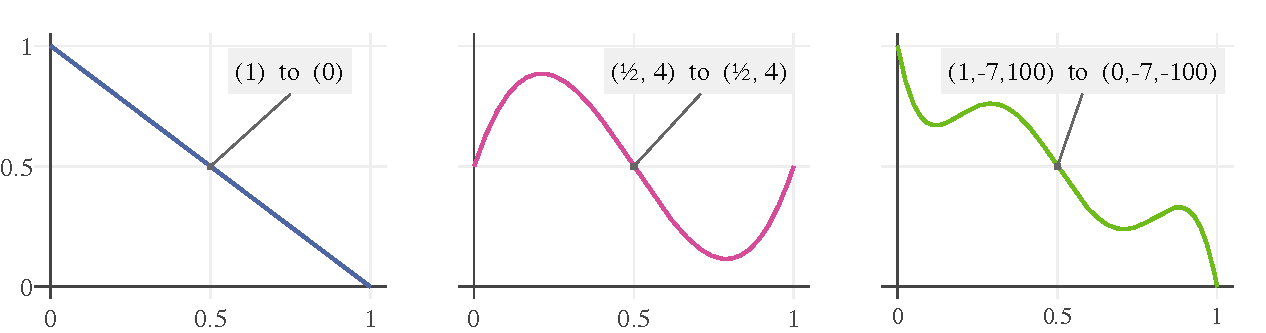
\includegraphics[width=.9\textwidth]{spline-demonstration}
  \caption{Example polynomials that interpolate function values at the ends of the interval $[0,1]$. The first only interpolates the function values $f(0) = 1$ and $f(1) = 0$, making it the order two polynomial $f(x) = 1 - x$. For the second plot $f(x) = 8x^3 - 12x^2 + 4x + 1/2$, which is order four and interpolates the values $f(0) = 1/2$, $f'(0) = 4$, $f(1) = 1/2$, $f'(1) = 4$. Finally the third plot shows the order six polynomial $f(x) = - 64x^5 + 160x^4 - 140x^3 + 50x^2 - 7x + 1$ interpolating the function values $f(0) = 1$, $f'(0) = -7$, $f''(0) = 100$, $f(1) = 0$, $f'(1) = -7$, $f''(1) = -100$. Notice that interpolating the same fixed number of function values at each endpoint will always result in an even order interpolating polynomial.
  }\label{fig:spline-demonstration}
\end{figure}

The importance of piecewise quintic interpolation over lower order approximations can be simply demonstrated. In general, the order of a polynomial determines the number of function values it can interpolate, and the growth rate of error away from the interpolated function values. As demonstrated in Figure \ref{fig:spline-demonstration}, it can be seen that matching a value at either end of the interval requires an order two (linear) approximation and each additional derivative at the ends of the interval raises the necessary polynomial order by two. The body of this work is composed of a novel algorithm for enforcing monotonicity on quintic polynomial pieces, then extending that solution to work on generic splines.

%% Software exists that does monotone piecewise quintic regression \cite{}, but the available routines do not computationally take advantage of the quintic monotonicity theory. ???

The major contribution of this work is an algorithm for constructing piecewise quintic Hermite interpolating polynomials that utilizes existing quintic monotonicity theory. The remainder of this paper is structured as follows: ...


\subsection{Computing a Monotone Cubic Interpolant}

The current state of the art monotone interpolating spline with a mathematical software implementation is piecewise cubic, continuously differentiable, and was first proposed in \cite{fritsch1980monotone} then expanded upon in \cite{carlson1985monotone}. Let $\pi: x_0 = k_1 < k_2 < \cdots < k_n = x_1$ be a partition of the interval $[x_0,x_1]$. Let $f: \mathbb{R} \rightarrow \mathbb{R}$ and $\{f(k_i) : i = 1,2,\ldots,n\}$ be a given set of data values at the partition points for a monotone function $f$, meaning $f(k_i) \leq f(k_{i+1})$ for $i = 1, \ldots, n-1$ or $f(k_i) \geq f(k_{i+1})$ for $i = 1, \ldots, n-1$. Let $\hat f$ be a piecewise cubic spline defined in each sub-interval $I_i = [k_i, k_{i+1}]$ by

\begin{align*}
h_i =& \ k_{i+1} - k_{i} \\
u(t) =& \ 3t^2 - 2t^3 \\
p(t) =& \ t^3 - t^2 \\
\hat f(x) =& \ f(k_i)\ u\big((k_{i+1} - x) / h_i\big) + f(k_{i+1})\ u\big((x - k_i) / h_i\big) \\
& - \hat f^{\ \prime}(k_i)\ p\big((k_{i+1}-x)/h_i\big) + \hat f^{\ \prime}(k_{i+1})\ p\big((x-k_i)/h_i \big).
\end{align*}

Notice that a trivially monotone spline results when $\hat f^{\ \prime}(k_i) = 0$, for $i = 1, \ldots, n$. However, such a spline has too many \textit{wiggles} for most applications. Fritsch and Carlson show that simple conditions on the derivative values can guarantee monotonicity, and that these conditions can be enforced in a way that ensures modifications on one interval will not break the monotonicity of cubic polynomials over any neighboring intervals. Consider the terms $\alpha = \big(\hat f^{\ \prime}(k_i) (k_{i+1}-k_i)\big) / \big(f(k_{i+1}) - f(k_i)\big)$ and $\beta = \big(\hat f^{\ \prime}(k_{i+1}) (k_{i+1}-k_i)\big) / \big(f(k_{i+1}) - f(k_i)\big)$, now monotonicity of a cubic polynomial over a sub-interval can be maintained by ensuring that $\alpha$ and $\beta$ reside in any of the regions depicted in Figure \ref{fig:projection}.

\begin{figure}
  \centering
  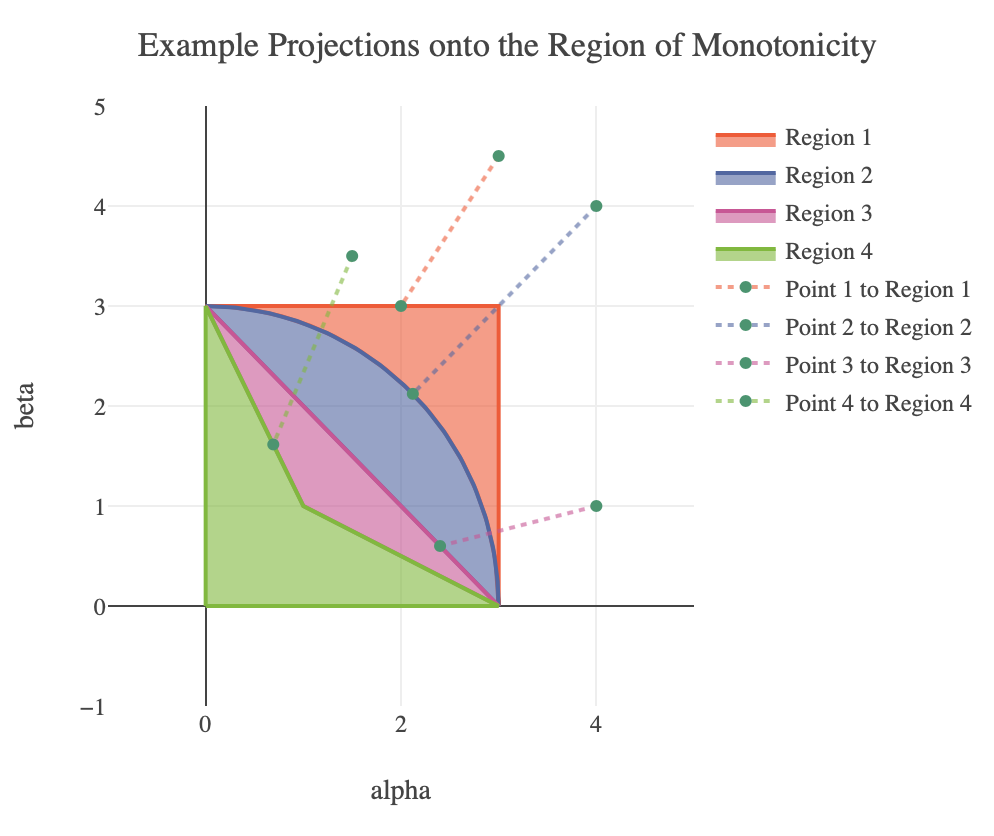
\includegraphics[width=0.50\textwidth]{demo_projection}
  \caption{These are the feasible regions of monotonicity for cubic splines and the projections that make a cubic polynomial piece monotone.}\label{fig:projection}
\end{figure}

The actual region of monotonicity for a cubic polynomial is larger, but projection of $(\alpha, \beta)$ into one of these regions ensures that monotonicity will be achieved and not violated for neighboring regions. The user must decide which region is most appropriate for the projections based on the application, Fritsch and Carlson recommend using region 2.

While the cubic monotonicity case affords such a concise solution, the region of monotonicity is not so simple in the quintic case. In the next section, an algorithm for performing a projection similar to those for cubic polynomials is proposed.

%% - show picture of how the cubic is computed
%% - show the algorithm for computing a cubic (and that it is trivial)
%% - quintic interpolation is more accurate when data is available, or higher order information can be inferred


\section{Monotone Quintic Interpolation}

The following section is composed of three algorithms that together are used to construct a piecewise quintic monotone interpolating spline. Section \ref{is_monotone} regards checking monotonicity, Section \ref{make_monotone} presents a procedure for enforcing monotonicity on a polynomial piece, and Section \ref{monotone_spline} combines the previous two algorithms into a routine for enforcing monotonicity over a quintic spline.

Similar to the cubic case, let $\pi: x_0 = k_1 < k_2 < \cdots < k_n = x_1$ be a partition of the interval $[x_0,x_1]$. Let $f: \mathbb{R} \rightarrow \mathbb{R}$ and $\{f(k_i) : i = 1,2,\ldots,n\}$ be a given set of values at the partition points for a monotone function $f$, meaning $f(k_i) \leq f(k_{i+1})$ or $f(k_i) \geq f(k_{i+1})$ for $i = 1, \ldots, n-1$.

In pseudo code, a function is used that is referred to as \texttt{line\_search($g,$ $a,$ $b$)}, where $a,$ $b$ $\in S$ for $S$ closed under convex combination, $g: S \rightarrow \{0,1\}$ is a binary function, and $g(b) = 1$. The \texttt{line\_search} is performed by Binary search in the presented framework, when $g(a) = 1$, $a$ is returned, otherwise the smallest $c \in [0,1]$ such that $g\big(a(1-c) + c b\big) = 1$ is returned.

In the case that first or second derivative information is not available at time of approximation, it is estimated with the central divided difference of the function values. The final quintic spline is represented with an exact rational arithmetic Newton Polynomial. % and evaluated with a B-spline basis.

\vspace{10pt}

%% ----------------------------------------------------------------------

\subsection{Verifying Monotonicity of a Quintic Polynomial}
\label{is_monotone}
Let $f$ be a quintic polynomial over a closed interval $[x_0, x_1]$ $\subset \mathbb{R}$. Now $f$ is uniquely defined by the evaluation tuples $\big(x_0,$ $f(x_0),$ $f'(x_0),$ $f''(x_0)\big)$ and $\big(x_1,$ $f(x_1),$ $f'(x_1),$ $f''(x_1)\big).$ Assume without loss of generality that $f(x_0) < f(x_1),$ where the case of monotonic decreasing $f$ would consider the negated the function values. The following algorithm will determine whether or not $f$ is monotone increasing on the interval $[x_0, x_1].$

\vspace{10pt}%
\hrule%
\vspace{3pt}%
\noindent\textbf{\textit{Algorithm 1:}} \texttt{is\_monotone$\big (x_0$,$x_1$,$f \big)$}%
\vspace{3pt}%
\hrule%

\begin{itemize}
  \itemsep0pt
  \parskip0pt

\item[1:] \texttt{if $\big(f(x_0) = f(x_1)\big)$ return $\big( Df(x_0) = Df(x_1) = D^2f(x_0) = D^2f(x_1) = 0 \big)$}
\item[2:] \texttt{if $\big(Df(x_0) < 0$ or $Df(x_1) < 0\big)$ return FALSE}
  \begin{itemize}
    \item[] \textit{This can be seen clearly from the fact that $f$ is analytic; there will exist some nonempty interval about $x_0$ or $x_1$ for which $Df$ is negative.}
  \end{itemize}


\item[2:] \texttt{if $\big(Df(x_0) = 0$ or $Df(x_1) = 0\big)$}
\item[3:] $\quad w = x_0 - x_1$
\item[4:] $\quad g(y) = \big({-4} Df(x_1) / w \big) < \big( ({-f}(x_1)/w - 24 y - 32 Df(x_1)) / 5w \big)$
\item[5:] $\quad$ \texttt{line\_search}$(g, 0, Df(x_0))$
\item[6:] $A = Df(x_0)\frac{x_1 - x_0}{f(x_1) - f(x_0)}$
\item[7:] $B = Df(x_1) \frac{x_1 - x_0}{f(x_1) - f(x_0)}$
  \begin{itemize}
    \item[] \textit{The variables $A$ and $B$ correspond directly to the theoretical foundation for positive quartic polynomials established in \cite{ulrich1994positivity}, first defined after equation 18.}
  \end{itemize}
\item[8:] $\gamma_0 = 4 \frac{Df(x_0)}{Df(x_1)} (B/A)^{3/4}$
\item[9:] $\gamma_1 = \frac{x_1 - x_0}{Df(x_1)} (B/A)^{3/4}$
\item[4:] $\alpha_0 = 4 (B/A)^{1/4}$
\item[5:] $\alpha_1 = -\frac{x_1 - x_0}{Df(x_1)} (B/A)^{1/4}$
\item[6:] $\beta_0 = 30 - \frac{12 \big(Df(x_0) + Df(x_1)\big) (x_1 - x_0)}{\big(f(x_1) - f(x_0)\big) \sqrt{A}\sqrt{B}}$
\item[7:] $\beta_1 = \frac{-3 (x_1 - x_0)^2}{2 \big(f(x_1) - f(x_0)\big) \sqrt{A} \sqrt{B}} $
  \begin{itemize}
    \item[] \textit{The $\gamma,$ $\alpha,$ and $\beta$ terms with subscripts $0$ and $1$ are algebraic reductions of the simplified conditions for satisfying Theorem 2 in \cite{ulrich1994positivity} (equation 16). These terms with subscripts $0$ and $1$ give the computation of $\alpha,$ $\beta,$ and $\gamma$ the form seen in lines $10$-$12$ below.}
  \end{itemize}
\item[10:] $\gamma = \gamma_0 + \gamma_1 D^2f(x_0)$
\item[11:] $\alpha = \alpha_0 + \alpha_1 D^2f(x_1)$
\item[12:] $\beta = \beta_0 + \beta_1 \big(D^2f(x_0) - D^2f(x_1)\big)$
\item[13:] \texttt{if $(\beta \leq 6)$ then return $\alpha > - (\beta + 2) / 2$}
\item[14:] \texttt{else return $\gamma > -2 \sqrt{\beta - 2}$ }

\end{itemize}
\hrule
\vspace{10pt}
%% ----------------------------------------------------------------------


%% ----------------------------------------------------------------------
Given the same initial conditions there are special circumstances which allow for the usage of simpler monotonicity conditions. In this case, consider when the quintic function has either $f'(x_0) = 0$ or $f'(x_1) = 0.$ This reduces the problem of verifying monotonicity to one of cubics established by \cite{schmidt1988positivity}.

\vspace{10pt}%
\hrule%
\vspace{3pt}%
\noindent\textbf{\textit{Algorithm 1b:}} \texttt{is\_monotone\_simplified}%
\vspace{3pt}%
\hrule%
\begin{itemize}
  \itemsep0pt
  \parskip0pt

\item[0:] $\alpha = 30 - \frac{(x_1 - x_0)\big( 14 f'(x_0) + 16 f'(x_1) - \big(f''(x_1) - f''(x_0) \big) (x_1 - x_0)\big)}{2\big(f(x_1) - f(x_0)\big)}$
\item[1:] $\beta = 30 - \frac{(x_1 - x_0)\big( 2 f'(x_0) + 24 f'(x_1) - \big(f''(x_0) + 3 f''(x_1) \big) (x_1 - x_0)\big)}{2\big(f(x_1) - f(x_0)\big)}$
\item[2:] $\gamma = \frac{(x_1 - x_0)\big( 7 f'(x_0) + f''(x_0) (x_1 - x_0) \big)}{f(x_1) - f(x_0)}$
\item[3:] $\delta = \frac{f'(x_0) (x_1 - x_0)}{f(x_1) - f(x_0)}$

  \begin{itemize}
    \item[] \textit{The variables above are algebraic expansions of the coefficients for the cubic derivative function in \cite{schmidt1988positivity}.}
  \end{itemize}

\item[4:] \texttt{if $\big($min$(\alpha, \delta) < 0\big)$ return FALSE}
\item[5:] \texttt{else if $\big(\beta < \alpha - 2 \sqrt{\alpha \delta}\big)$ return FALSE}
\item[6:] \texttt{else if $\big(\gamma < \delta - 2 \sqrt{\alpha \delta}\big)$ return FALSE}
\item[7:] \texttt{else return TRUE}

\end{itemize}
\hrule
\vspace{10pt}
%% ----------------------------------------------------------------------

Next the modification of a quintic spline to enforce monotonicity will be discussed.

%% ----------------------------------------------------------------------
\subsection{Enforcing Monotonicity of a Quintic Polynomial}
\label{make_monotone}

\vspace{10pt}%
\hrule%
\vspace{3pt}%
\noindent\textbf{\textit{Algorithm 2a:}} \texttt{make\_monotone}%
\vspace{3pt}%
\hrule%

\begin{itemize}
  \itemsep0pt
  \parskip0pt

\item[0:] \texttt{if }$\big(f(x_1) - f(x_0) = 0\big)$ \texttt{ return } $f'(x_0) = f'(x_1) = f''(x_0) = f''(x_1) = 0$
\item[1:] $f'(x_0) = \ $\texttt{median}$\big(0, f'(x_0), 14 \frac{f(x_1) - f(x_0)}{x_1 - x_0} \big)$
\item[2:] $f'(x_1) = \ $\texttt{median}$\big(0, f'(x_1), 14 \frac{f(x_1) - f(x_0)}{x_1 - x_0}\big)$
  \begin{itemize}
  \item[] \textit{This selection of values for $f'(x_0)$ and $f'(x_1)$ is suggested by \cite{ulrich1994positivity} (originally from \cite{huynh1993accurate}), and quickly enforces upper and lower bounds on derivative values to ensure quintic monotonicity is obtainable.}
  \end{itemize}
\item[3:] $A = f'(x_0)\frac{x_1 - x_0}{f(x_1) - f(x_0)}$
\item[4:] $B = f'(x_1) \frac{x_1 - x_0}{f(x_1) - f(x_0)}$
\item[5:] \texttt{if }$AB \leq 0$\texttt{ return make\_monotone\_simplified}
\item[6:] \texttt{if $\big($max}$(A,B) > 6\big)$\\$f'(x_0) = 6 f'(x_0)\  /$\texttt{ max}$(A,B)$\\$f'(x_1) = 6 f'(x_1)\  /$\texttt{ max}$(A,B)$

  \begin{itemize}
  \item[] \textit{This box bound ensures that $(A,B)$ remains within a viable region of monotonicity (satisfying Theorem 4, seen in Fig. 6 of \cite{ulrich1994positivity}).}
  \end{itemize}

\item[7:] $f''(x_0) = - \sqrt{A} \big( 7 \sqrt{A} + 3 \sqrt{B} \big) \frac{f(x_1) - f(x_0)}{(x_1 - x_0)^2}$\\$f''(x_1) = \sqrt{B} \big( 3 \sqrt{A} + 7 \sqrt{B} \big) \frac{f(x_1) - f(x_0)}{(x_1 - x_0)^2}$

  \begin{itemize}
    \item[] \textit{This selection of values of $f''$ is guaranteed to satisfy Theorem 4 from \cite{ulrich1994positivity} and is chosen because it is (reasonably) the average of the two endpoints of the interval of monotonicity for second derivative values.}
  \end{itemize}

\item[8:] $\eta = \big(f''(x_0), f''(x_1)\big)$\\$\eta_0 = \big(f''(x_0), f''(x_1)\big)$\\$f''(x_0), f''(x_1) = $\texttt{ line\_search$\big($is\_monotone, $\eta,$ $\eta_0\big)$}
\end{itemize}
\hrule
\vspace{10pt}
%% ----------------------------------------------------------------------


Similar to the simplified check for monotonicity, when the derivative value at one endpoint of the interval is $0$, a simplified set of steps can be taken to enforce monotonicity.

%% ----------------------------------------------------------------------
\vspace{10pt}%
\hrule%
\vspace{3pt}%
\noindent\textbf{\textit{Algorithm 2b:}} \texttt{make\_monotone\_simplified}%
\vspace{3pt}%
\hrule%

\begin{itemize}
  \itemsep0pt
  \parskip0pt

\item[0:] $f''(x_0) = $\texttt{ max}$\bigg(f''(x_0), \frac{-6 f'(x_0)}{x_1 - x_0}\bigg)$

  \begin{itemize}
    \item[] \textit{Considering the $\alpha,$ $\gamma,$ $\beta,$ and $\delta$ defined in \cite{schmidt1988positivity}, this first step enforces $\gamma > \delta.$ It is already guaranteed that $\delta = \frac{f'(x_0)(x_1 - x_0)}{f(x_1) - f(x_0)} > 0.$ Only two conditions remain to guarantee monotonicity.}
  \end{itemize}

\item[1:] $f''(x_1) = $\texttt{ max}$\bigg( f''(x_1), f''(x_0) + \frac{14 f'(x_0) + 16 f'(x_1) + 60(f(x_1) - f(x_0)) / (x_1 - x_0)}{x_1 - x_0} \bigg)$

  \begin{itemize}
    \item[] \textit{Now it is guaranteed that $\alpha \geq 0.$}
  \end{itemize}

\item[2:] $f''(x_1) = $\texttt{ max}$\bigg( f''(x_1), 6 f'(x_0) - 4 f'(x_1) - f''(x_0) \bigg)$

  \begin{itemize}
    \item[] \textit{Lastly, this guarantees that $\beta \geq \alpha.$ All conditions are met to satisfy proposition 2 of \cite{schmidt1988positivity} and ensure monotonicity.}
  \end{itemize}
\end{itemize}
\hrule
\vspace{10pt}
%% ----------------------------------------------------------------------
Notice that all above algorithms (assuming a fixed level of precision is desired) have $\mathcal{O}(1)$ runtime. Only a finite number of operations are needed for monotonicity verification. A line search is performed for enforcement, however that search requires a fixed number of steps to achieve any predetermined relative precision on the line.


%% ----------------------------------------------------------------------
\subsection{Constructing a Piecewise Quintic Monotone Spline}
\label{monotone_spline}

Finally, the construction of a full piecewise quintic spline is outlined using the above algorithms. Let $f: \mathbb{R} \rightarrow \mathbb{R}$ be a function in $\mathcal{C}^2.$ Proceed given evaluation tuples $\big(x_i,$ $f(x_i),$ $f'(x_i),$ $f''(x_i)\big)$ for $i = 0,\ldots,N$ such that $x_i < x_{i+1}$ and (without loss of generality) $f(x_i) \leq f(x_{i+1})$ for $i = 1,$ $\ldots,$ $N-1$. 

\vspace{10pt}%
\hrule%
\vspace{3pt}%
\noindent\textbf{\textit{Algorithm 3:}} \texttt{monotone\_spline}%
\vspace{3pt}%
\hrule%

\begin{itemize}
  \itemsep0pt
  \parskip0pt

\item[0:] \texttt{for }$i=0,\ldots,N-1$
\item[1:] $\quad$\texttt{if $\big($not is\_monotone$(i,i+1)\big)$  make\_monotone$(i,i+1)$}

  \begin{itemize}
    \item[] \textit{In the shorthand notation above, $i$ and $i+1$ refer to the associated tuples of the form $(x_i,$ $f(x_i),$ $f'(x_i),$ $f''(x_i)).$ This notation will be used through the remainder of this algorithm.}
  \end{itemize}

\item[2:] $\quad$\texttt{for $j=i-1,\ldots,0$}
\item[3:] $\quad\quad$\texttt{if $\big($not is\_monotone$(j,j+1)\big)$  make\_monotone$(j,j+1)$}
\item[4:] $\quad\quad$\texttt{else break}

  \begin{itemize}
    \item[] \textit{The above `for' loop will be referred to as the cascade fix. If the adjustment of second derivative values causes the previous interval to become nonmonotone, then the left-hand second derivative value must be updated. This may (abnormally) require adjustments across all previously visited intervals.}
  \end{itemize}

\item[5:] $\quad$\texttt{while $\big($not is\_monotone$(i,i+1)\big)$}
\item[6:] $\quad\quad f'(x_i) = f'(x_i) / k$
\item[7:] $\quad\quad f'(x_{i+1}) = f'(x_{i+1}) / k$
\item[8:] $\quad\quad$\texttt{make\_monotone$(i,i+1)$}

  \begin{itemize}
    \item[] \textit{In the case that the two corrections to neighboring intervals contradict, the first derivative values of the active interval are decreased to enlarge the overlap of regions I and II (from \cite{ulrich1994positivity}) of the two intervals.}
  \end{itemize}

\item[9:] $\quad\quad$\texttt{for $j=i-1,\ldots,0$}
\item[10:] $\quad\quad\quad$\texttt{if $\big($not is\_monotone$(j,j+1)\big)$  make\_monotone$(j,j+1)$}
\item[11:] $\quad\quad\quad$\texttt{else break}

  \begin{itemize}
    \item[] \textit{Finally an additional `cascade fix' is performed to ensure that all previous intervals are still monotone after shrinking the derivative values of the current interval.}
  \end{itemize}

\end{itemize}
\hrule
\vspace{10pt}
%% ----------------------------------------------------------------------

It is mentioned in \cite{ulrich1994positivity} that for sufficiently small $f'(x_i)$ and $f'(x_{i+1})$ the admissible solution interval of second derivative values becomes arbitrarily large. It can also be seen that decreasing the assigned derivative on right-hand side of an interval always allows the achievement of monotonicity because shrinking $f'(x_1)$ results in $\gamma$ growing faster than $\sqrt{\beta}$ for \textit{algorithm 1a}, for \textit{algorithm 1b} $\beta$ and $\gamma$ will grow faster $\alpha$ and $\delta$ respectively. In application, one needs only to pick some $k > 1$ to ensure successful termination.

Given the potential for successive cascade fixes, the runtime of \textit{algorithm 3} is $\mathcal{O}(N^2)$. In practice this has been observed to be incredibly unlikely and difficult to produce. While single cascade fixes can occur from hand crafted examples, the generously rounded values selected to ensure monotonicity frequently prevent successive cascade fixes.

%% - background is provided by these papers

%% - Table of relevant terms and what they mean

%% \subsection{Algorithm: Monotone Quintic Interpolation}
%% - correctness of algorithm
%% - runtime of algorithm
%% - weakness of algorithm



\section{Experimental Results}

- show a Figure of a simple quintic interpolant and its derivatives

\subsection{Approximating a Trigonometric Function}

For this experiment, the function $\sin(x) + x$ is considered over the
interval $[0,(5/2)\pi]$.

\begin{figure}[htb]
  \centering
  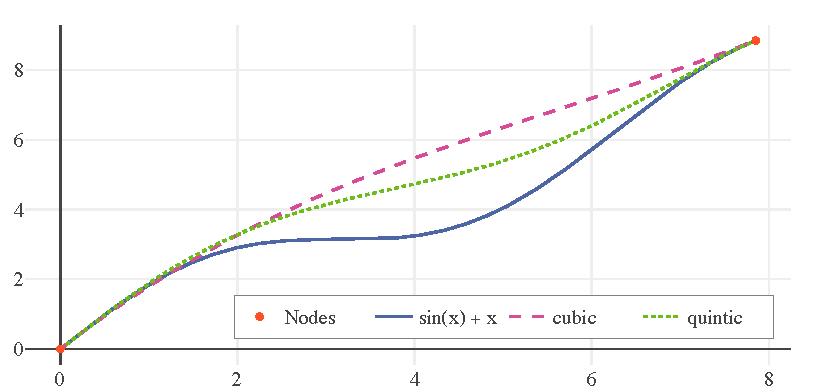
\includegraphics[width=.7\textwidth]{cubic-quintic-sin}
  \caption{Depicted above are the monotone cubic and quintic spline
    interpolant of the function $\sin(x) + x$ over the nodes $[0,
      (5/2) \pi]$.  Notice that the maximum error of the cubic
    interpolant is larger, because it only captures first derivative
    information at the nodes. The quintic interpolant captures both
    first and second derivative information at the nodes.
  }\label{fig:cubic-quintic-sin}
\end{figure}


- Pick a trig function, approximate it with cubic and quintic

- Show a Figure, and a Table of the maximum error and distribution of
  error across the segment

\subsection{Approximating a Cumulative Distribution Function}

- generate large sets of random monotone data, show Table of number
  of metrics growing with increasing number of nodes

- show visual of the \textit{error} 

\subsection{Random Monotone Data}

- generate large sets of random monotone data, show Table of number
  of metrics growing with increasing number of nodes (how many binary
  searches, how many corrections were needed, steps were taken)

\section{Discussion}

- this algorithm has its quirks, but it works

- this is an improvement over the cubic, although the complexity of
  the algorithm is greatly increased as well

\section{Future Work}

- a method for finding regions of monotonicity that is less ad-hoc 

- constructing monotone interpolants for higher order approximations

- using improved distribution estimates to improve distribution modeling

\section{Conclusion}

- this paper proposes and tests an algorithm for constructing quintic
  monotone interpolants

- the results show an improvement over the cubic usage




\section*{Acknowledgments}
The NSF is acknowledged for its support of this project.

% Please don't change the bibliographystyle style
\bibliographystyle{scsproc}
% AUTHOR: Include your bib file here
\bibliography{paper}


\section*{Author Biographies}

\textbf{\uppercase{THOMAS C. H. LUX}} is a Ph.D. candidate in Computer Science at Virginia Polytechnic Institute and State University. His research interests include Computational Science, Approximation Theory, Optimization, and Artificial Intelligence. His email address is \email{tchlux@vt.edu}.

\newpage

\appendix

\section{Author Checklist}
We strive for a consistent appearance in all papers published in the proceedings. If you used the template and styles within this author’s kit, then almost all of the requirements in this checklist will be automatically satisfied, and there is very little to check.

Please \textbf{print a hardcopy of your paper}, and go over your printed paper to make sure it adheres to the following requirements. \textit{Thank you!}

\begin{enumerate}
	\item Abstract
  \begin{enumerate}
	  \item 150 or fewer words.
	  \item Provide 3-5 keywords (mandatory). This set of keywords will identify your paper in indices and databases.
	\end{enumerate}
	\item Paper Length
  \begin{enumerate}
	  \item At least 5, but no more than 12 pages.
	  \item Page size is letter size (8.5’’ x 11’’, or 216 mm x 279 mm).
	\end{enumerate}
	\item All text is in 11-Point Times New Roman except title, header and footer (default in this template).
	\item Paper title is in 12-Point Times New Roman \textbf{BOLDFACE ALL CAPS} (default in this template).
	\item The paper has been spellchecked using U.S. English. 
	\item Spacing and Margins
  \begin{enumerate}
	  \item Single spaced.
	  \item Left and right margins are each 1 inch (default in this template).
	  \item Top and bottom margins are according to the template.
	  \item Title starts 1.25 inches from the top of the page (default in this template).
	\end{enumerate}
	\item Section Headings
  \begin{enumerate}
	  \item Left justified and set in \textbf{BOLDFACE ALL CAPS} (default in this template).
	  \item Numbered, except for the abstract, acknowledgments, references and author biographies.
	  \item Subsection headings are set in \textbf{Boldface Headline Style} (default in this template).
	\end{enumerate}
	\item No footnotes or page numbers.
	\item The copyright notice on the first page contains the name of the symposium or a track where you want to submit your paper, and the running head on subsequent pages is the surnames of all authors.
	\item Multiple authors are formatted correctly.
	\item Equations are centered and any equation numbers are in parentheses and right-justified (default).
	\item Figures and Tables
  \begin{enumerate}
	  \item All text in figures and tables is readable.
	  \item Table captions appear above the table.
	  \item Figure captions appear below the figure.
	\end{enumerate}
	\item Citations and References
  \begin{enumerate}
	  \item Citations are by author and year, and are enclosed in parentheses, not brackets (default \BibTeX). 
	  \item References are in the hangref style, and are listed alphabetically by the last names(s) of the author(s) (also default \BibTeX\ setting in this template). 
	\end{enumerate}
	\item Author biographies are one paragraph per author.
	\item Hyperlinks
  \begin{enumerate}
	  \item Be sure that hyperlinks will probably work in the future as well.
	  \item Live hyperlinks are blue. Nonlive hyperlinks are black (default in this template).
	\end{enumerate}
	\item All fonts must be embedded in the resulting \texttt{.pdf}. If you use \texttt{pdflatex}, this should already be true--unless you included figures in the \texttt{.eps} or \texttt{.pdf} format which may introduce additional font dependencies. You can use the \texttt{pdffonts} command to see if all the fonts are embedded (the column ``emb'' should say yes for all rows). You can use GhostScript to force embed the fonts, like so: {\texttt{gs -dNOPAUSE -dBATCH -sDEVICE=pdfwrite -dEmbedAllFonts=true -sOutputFile=out.pdf -f in.pdf}} (in Windows, use \texttt{gswin32} or \texttt{gswin32c} to invoke GhostScript).
\end{enumerate}

After verifying that your paper meets these requirements, please go to the final submission page at conference website and submit your paper. Be sure to complete the transfer of copyright form and upload the \texttt{.pdf} receipt. \textit{Thank you for contributing to the SCS conferences!}

\section{Most Observed Mistakes}

The following list comprises \textbf{the most common sources of error} that had to be corrected by previous editors. Please make sure to go through the following list and check that your paper is formatted correctly:
\begin{enumerate}
	\item	The paper is less than 5 or more than 12 pages long.
	\item	Paper title and section titles are in \textbf{BOLD ALL CAPS}, subsections are \textbf{Bold and Capitalize the First Letter of Important Words}. Please use the templates.
	\item	Paper is in A4 format, not letter format. Please use the required margins.
	\item	The copyright notice is incorrect.
	\item	The running heads are incorrect. Do not forget that the LastNameLastAuthor is preceded by ``, and ''.
	\item	The citation format is incorrect. Use \BibTeX\ for citations and do not change the format used by the template.
	\item	The biographies are missing. Do not forget the ``author biographies'' section.
	\item	Figures or tables are not referenced in the text or have the incorrect caption format.
	\item	The author section after the title is not formatted correctly, the number of organizations does not define the number of blocks, or the number of blocks does not define the layout.
	\item In the heading on the title page, country names are in all capitals.
	\item	Paragraphs are not indented.
	\item Some fonts in the resulting \texttt{.pdf} are not embedded.
\end{enumerate}



\end{document}
